\begin{homeworkProblem}
    The following complex numbers are expressed as $\lambda=a+bi$, where $a$ is the
    real part and $b$ is the imaginary part. Express the nubmer in polar form
    $\lambda = re^{i\theta}$, and use your result to compute the indicated power
    $\lambda^n$ of this complex number. Sketch $\lambda^n$, for $n = 0, 1, 2, 3, 4$
    as a function of $n$.
    \begin{multicols}{2}
        \begin{enumerate}
            \item $1+i$
            \item $1-i$
            \item $10i$
            \item $-1+\sqrt{3}i$
            \item $-\frac{1}{2} - \frac{i}{2}$
            \item[\vspace{\fill}] % placeholder
        \end{enumerate}
    \end{multicols}
    
    \segline
    
    \solution
    
    \begin{multicols}{2}
    \begin{enumerate}
    
    % Solution 8(a)
    \item \textbf{Polar form}:
    $\begin{aligned}
        z^n &= (\sqrt{1^2 + 1^2} e^{i\tan^{-1}(1)})^n\\ &= (\sqrt{2})^n e^{i\pi n/4}
    \end{aligned}$.
    \begin{figure}[H]
        \centering
        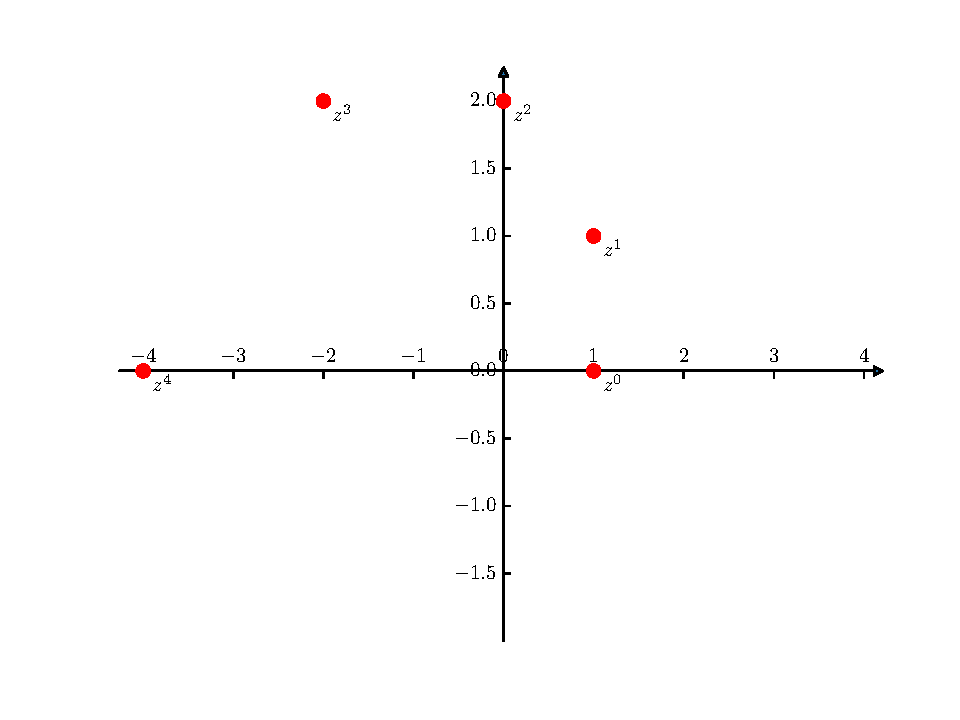
\includegraphics[scale=0.5]{fig/fig8(a).pdf}
    \end{figure}
    
    % Solution 8(b)
    \item \textbf{Polar form}:
    $\begin{aligned}
        z^n &= (\sqrt{1^2 + (-1)^2} e^{i\tan^{-1}(-1)})^n\\
        &= (\sqrt{2})^n e^{-i\pi n/4} (\cos > 0\& \sin < 0)
    \end{aligned}$.
    \begin{figure}[H]
        \centering
        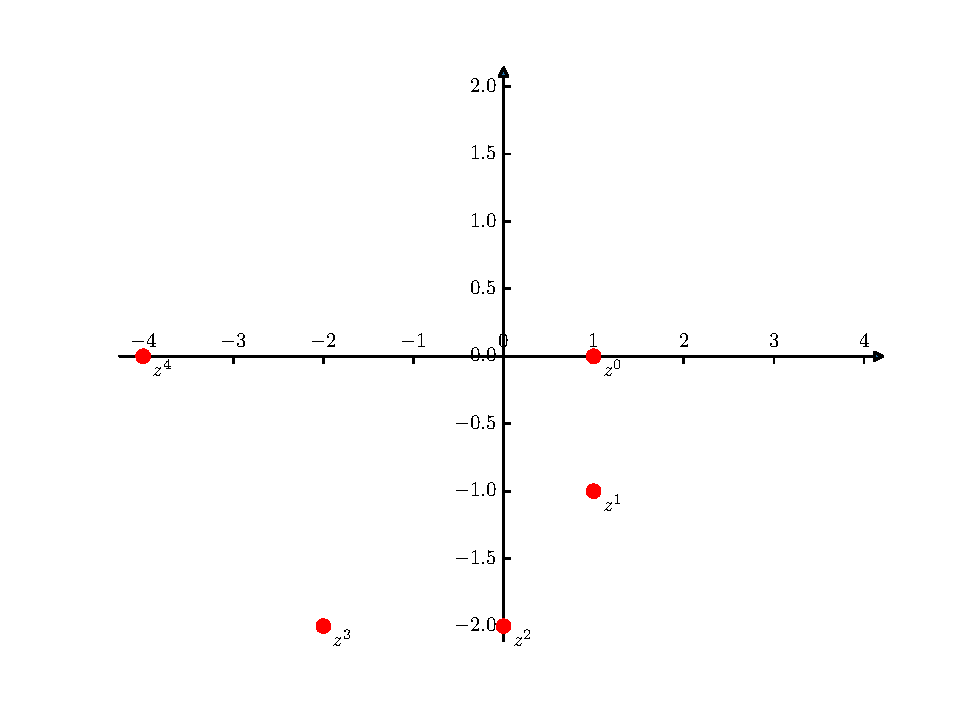
\includegraphics[scale=0.5]{fig/fig8(b).pdf}
    \end{figure}
    
    % Solution 8(c)
    \item \textbf{Polar form}:
    $\begin{aligned}
        z^n &= (\sqrt{0^2 + 10^2} e^{i\tan^{-1}(10/0)})^n\\ &= 10^ne^{i\pi n/2}
    \end{aligned}$.
    \begin{figure}[H]
        \centering
        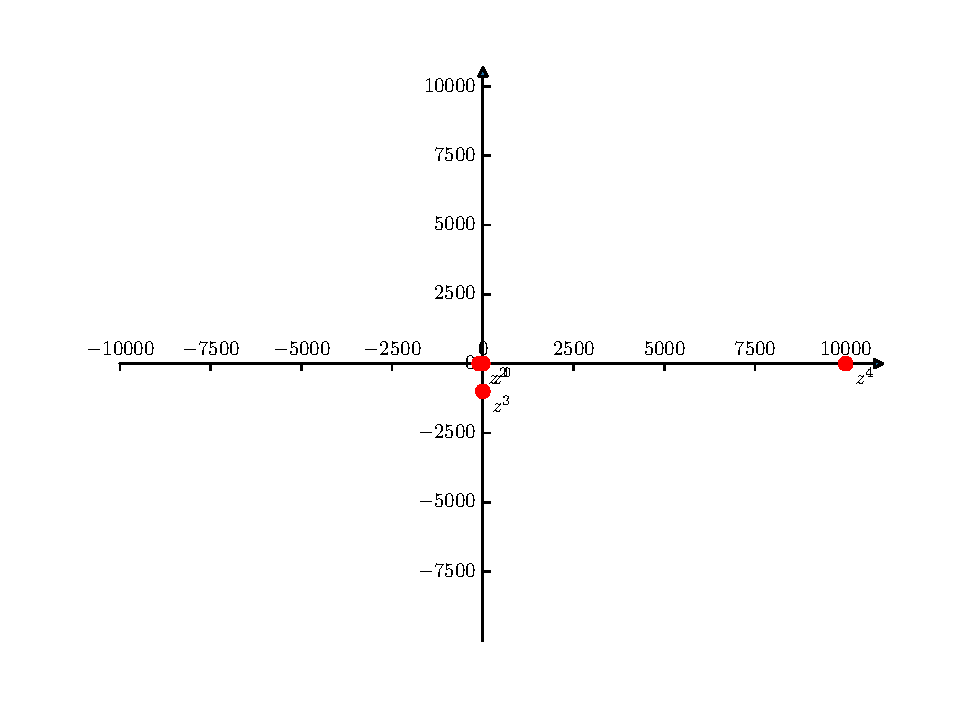
\includegraphics[scale=0.5]{fig/fig8(c).pdf}
    \end{figure}
    
    % Solution 8(d)
    \item \textbf{Polar form}:
    $\begin{aligned}
        z^n &= (\sqrt{(-1)^2 + (\sqrt{3})^2} e^{i\tan^{-1}(-\sqrt{3})})^n\\
        &= 2^n e^{2i\pi n/3}
    \end{aligned}$
    \begin{figure}[H]
        \centering
        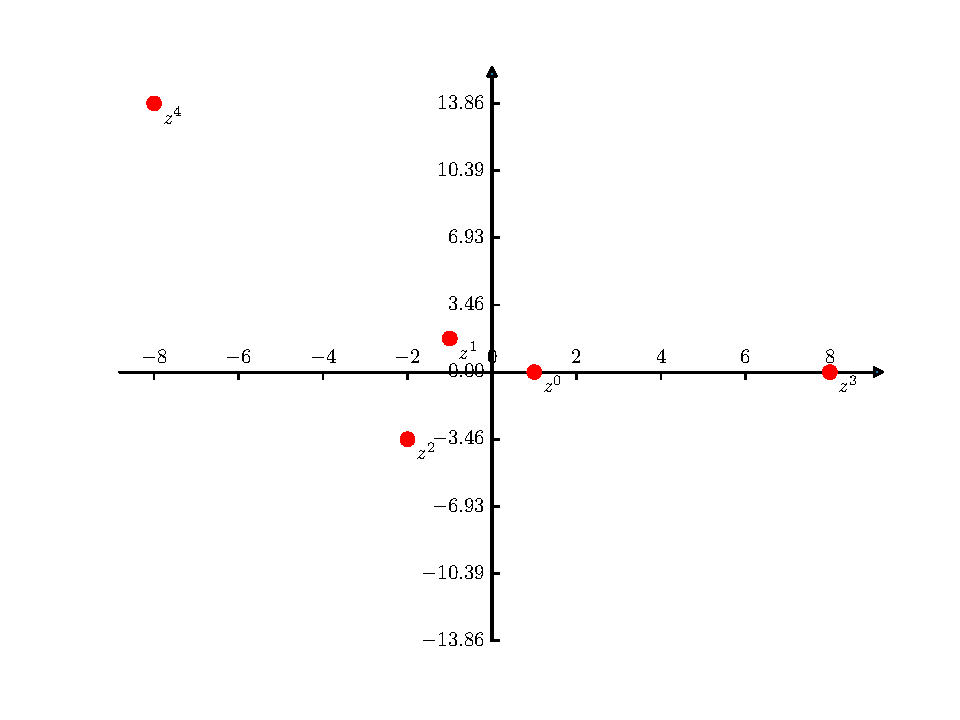
\includegraphics[scale=0.5]{fig/fig8(d).pdf}
    \end{figure}
    % Solution 8(e)
    \item \textbf{Polar form}:
    $\begin{aligned}
        z^n &= (\sqrt{(-1/2)^2+(-1/2)^2} e^{i\tan^{-1}(1)})^n\\
        &=(\frac{1}{\sqrt{2}})^n e^{i5\pi n/4} (\sin \& \cos < 0)
    \end{aligned}$.
    \begin{figure}[H]
        \centering
        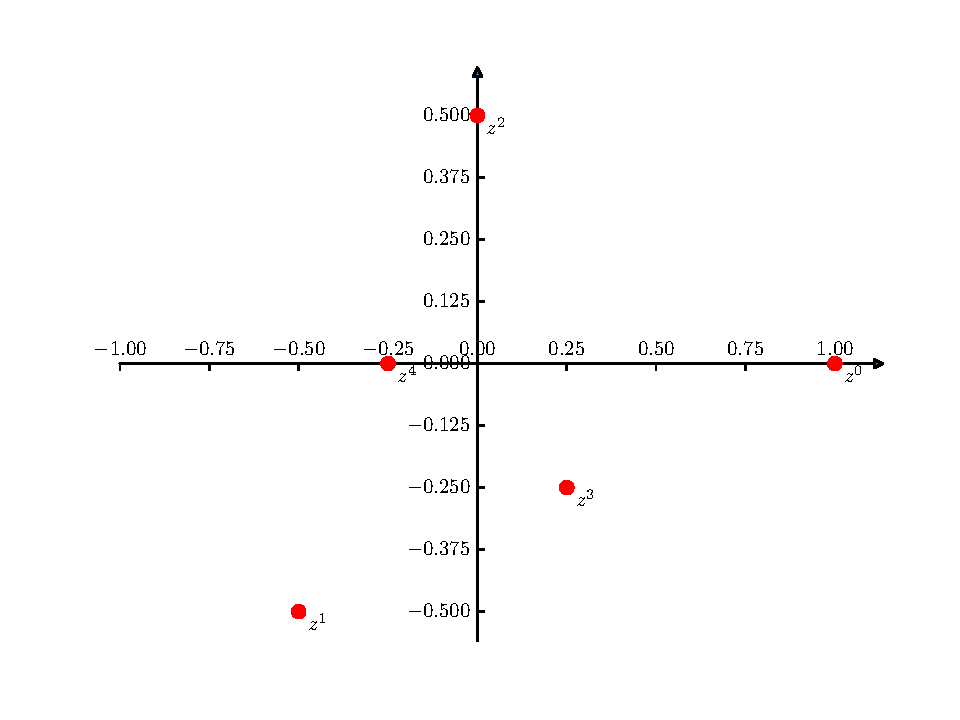
\includegraphics[scale=0.5]{fig/fig8(e).pdf}
    \end{figure}
    
    \end{enumerate}
    \end{multicols}
    \end{homeworkProblem}